% =============================================================================
%  Trabalho Prático 2 - Fundamentos de Inteligência Artificial (UFMG / DEE)
%  Busca local e algoritmo genético no sequenciamento de manutenção de ativos
%
%  Compilar com pdfLaTeX (Overleaf: Menu -> Compiler: pdfLaTeX; Main document:
%  main.tex). Localmente: `make report`.
%
%  As tabelas (tabelas/*.tex) e as figuras (figuras/*.pdf) são geradas por
%  `make analysis` a partir dos CSVs em results/. Não edite esses arquivos à
%  mão: mude o código de análise e gere de novo.
% =============================================================================
\documentclass[10pt,a4paper]{article}

\usepackage[T1]{fontenc}
\usepackage[utf8]{inputenc}
\usepackage[brazil]{babel}
\usepackage{lmodern}
\usepackage{microtype}
\usepackage[a4paper,margin=2cm]{geometry}
\usepackage{amsmath,amssymb}
\usepackage{graphicx}
\usepackage{booktabs}
\usepackage{caption}
\usepackage{float}
\usepackage{verbatim}
\usepackage{textcomp}
\usepackage{natbib}
\usepackage{flafter}
\usepackage[hidelinks]{hyperref}

\graphicspath{{figuras/}}
\captionsetup{font=small,labelfont=bf}
\setlength{\tabcolsep}{3.5pt}
\setlength{\textfloatsep}{10pt plus 2pt minus 2pt}
\setlength{\floatsep}{8pt plus 2pt minus 2pt}
% Deixa tabelas e figuras dividirem a página com o texto (evita páginas só de floats).
\renewcommand{\topfraction}{0.9}
\renewcommand{\bottomfraction}{0.8}
\renewcommand{\textfraction}{0.07}
\renewcommand{\floatpagefraction}{0.8}

% Tabelas geradas: só o tabular, centralizado e em fonte menor.
\newcommand{\tabela}[1]{{\small\centering\input{tabelas/#1}\par}}

\title{\textbf{Busca Local e Algoritmo Genético no\\Sequenciamento de Manutenção de Ativos}\\[0.5em]
       \large Trabalho Prático 2 -- Fundamentos de Inteligência Artificial}
\author{Arthur Fernandes\\{\small Matrícula 2020026800} \and Bruno Lima\\{\small Matrícula 2022055785}}
% TODO grupo: confirmar se Felipe Augusto faz parte do grupo neste TP e incluir o nome.
\date{Universidade Federal de Minas Gerais -- Departamento de Engenharia Elétrica\\
      Profs. Cristiano Leite de Castro e João Pedro Campos\\[0.5em]
      Outubro de 2026}

\begin{document}

\maketitle

\begin{abstract}
\noindent
Comparamos três metaheurísticas no sequenciamento de manutenção de $n$ ativos por uma única equipe, com custo igual ao atraso total ponderado: descida gulosa com reinício aleatório, \textit{simulated annealing} (SA) e um algoritmo genético (AG).
Todas usam a mesma interface e o mesmo orçamento de avaliações de $h$, com parada exata, em três instâncias ($n = 12$, $50$ e $150$).
A vizinhança de inserção venceu a troca e o 2-opt e foi adotada.
A descida gulosa e o SA ficaram estatisticamente empatados nas três instâncias e venceram o AG em todas elas (Mann--Whitney com correção de Holm, $p \le 0{,}015$).
Na instância pequena, as duas buscas locais acharam o ótimo $h^* = 1\,875$ em 30 de 30 execuções; o AG, em 12.
O AG perde diversidade cedo: na instância média nenhuma execução melhora depois da metade do orçamento.
No experimento extra, trocar o cruzamento OX por PMX, por mutação pura ou por cruzamento com indivíduos aleatórios não melhorou o AG; só a busca local nos filhos (AG memético) o levou ao nível das buscas locais, sem superá-las.
Na instância média, o AG memético encontrou $h = 16\,234$, abaixo do melhor valor conhecido (16\,332).
\end{abstract}

\section{Introdução}
\label{sec:introducao}

Uma equipe parte da base em $(50, 50)$ e precisa visitar $n$ ativos da rede de distribuição, cada um com tempo de serviço $p_j$, prazo regulatório $d_j$ e peso $w_j$~\citep{enunciado2026tp2}.
O deslocamento entre dois pontos leva a distância euclidiana arredondada, e não há retorno à base.
Uma solução é a ordem de visita, uma permutação $\pi$ dos ativos, e o custo é o atraso total ponderado
\begin{equation}
  h(\pi) = \sum_{j=1}^{n} w_j \max\left(0,\; C_j - d_j\right),
  \label{eq:custo}
\end{equation}
em que $C_j$ é o instante em que o serviço do ativo $j$ termina.
Toda permutação é viável, então o problema é de otimização pura sobre $n!$ pontos, com $4{,}8 \times 10^{8}$ soluções já na instância pequena.

O enunciado fixa o orçamento $B$ de avaliações de $h$ e o número de execuções independentes de cada instância (Tabela~\ref{tab:instancias}).
Os dois critérios gulosos naturais puxam em direções opostas: visitar o mais próximo economiza deslocamento, e visitar o mais urgente evita multa.
O guloso do enunciado, que escolhe o menor acréscimo imediato de atraso, chega a $3\,168$ na instância pequena, 69\% acima do ótimo.

\begin{table}[tbp]
  \centering\small
  \caption{Instâncias, orçamento e valores de referência do enunciado. Só o valor da pequena é ótimo comprovado.}
  \label{tab:instancias}
  \begin{tabular}{lrrrrr}
    \toprule
    Instância & $n$ & $\sum p_j$ & Orçamento $B$ & Execuções & $h_{\mathrm{ref}}$ \\
    \midrule
    pequena & 12 & 55 & 50\,000 & 30 & 1\,875 (ótimo) \\
    média & 50 & 239 & 150\,000 & 30 & 16\,332 \\
    grande & 150 & 684 & 300\,000 & 10 & 60\,417 \\
    \bottomrule
  \end{tabular}
\end{table}

A Seção~\ref{sec:implementacao} descreve as decisões de implementação que afetam a comparação.
As Seções~\ref{sec:t1} a~\ref{sec:t3} trazem as tarefas T1 a T3, e a Seção~\ref{sec:discussao} responde às quatro perguntas obrigatórias, incluindo o experimento extra.
Os comandos que reproduzem cada tabela e figura estão no Apêndice~\ref{ap:reproducao}.

\section{Implementação}
\label{sec:implementacao}

\paragraph{Algoritmo separado do problema.}
Os algoritmos enxergam o problema só pela interface sugerida no enunciado (\texttt{solucao\_aleatoria}, \texttt{h}, \texttt{sucessores}, \texttt{sucessor\_aleatorio}, \texttt{cruzamento}, \texttt{mutacao}), com uma extensão.
Em vez da permutação pronta, \texttt{sucessores} devolve pares (movimento, $h$ do sucessor), e um método \texttt{aplicar} constrói o sucessor só quando o algoritmo o aceita.
O movimento é opaco para o algoritmo, e sem essa extensão a avaliação incremental exigiria montar cada sucessor inteiro antes de avaliá-lo.
Um teste automático falha se algum algoritmo importar o módulo do problema.

\paragraph{Contagem de avaliações.}
Um invólucro em volta do problema conta toda avaliação de $h$: chamadas diretas, cada sucessor examinado e cada filho do AG.
A avaliação $B+1$ lança uma exceção que encerra o algoritmo, que portanto nunca checa o orçamento por conta própria.
A descida gulosa não recalcula o $h$ da solução corrente; ele vem do sucessor aceito.
Ao fim de cada execução conferimos que foram exatamente $B$ avaliações e reavaliamos a melhor permutação num problema sem contador; as duas condições valeram em todas as execuções.

\paragraph{Vizinhanças e avaliação incremental.}
A troca (\textit{swap}) e o 2-opt geram $n(n-1)/2$ sucessores distintos, e a inserção gera $(n-1)^2$, porque mover o elemento da posição $i$ para $i+1$ equivale a mover o de $i+1$ para $i$.
Um movimento não altera as posições anteriores à primeira que toca.
Guardamos então, para a solução corrente, o instante de conclusão e o custo acumulados em cada posição, e avaliamos cada sucessor a partir desse prefixo.
Testes de propriedade (150 instâncias aleatórias, mais todos os sucessores da pequena e da média) confirmam que o valor incremental é idêntico ao completo.
O ganho medido em $n = 150$ fica entre 1,38 e 1,45 vezes (Tabela~\ref{tab:t2}).
É pouco porque a primeira posição tocada cai em média em $n/3$: ainda é preciso refazer cerca de $2n/3$ das posições, o que limita o ganho a uns 1,5 vezes.

\paragraph{Descida gulosa.}
As três variantes estão implementadas.
A \textit{best improvement} examina a vizinhança inteira e fica com o melhor sucessor; a \textit{first improvement} percorre a vizinhança em ordem aleatória e aceita o primeiro que melhora; a \textit{random} sorteia sucessores e aceita o primeiro que melhora.
Como a \textit{random} não tem como provar que chegou a um ótimo local, ela recomeça depois de $K = |N(s)|$ sorteios seguidos sem melhoria.
Com reposição, a chance de nunca sortear um movimento de melhoria específico nesses $K$ sorteios é $(1 - 1/K)^K \approx e^{-1} \approx 37\%$.

\paragraph{Simulated annealing.}
O SA aceita um sucessor que não piora e aceita uma piora $\Delta > 0$ com probabilidade $e^{-\Delta/T}$~\citep{kirkpatrick1983annealing,slides2026cap4}.
O resfriamento é geométrico em patamares de $L$ passos, e $\alpha = (T_f/T_0)^{1/(M-1)}$, com $M = \lceil (B-1)/L \rceil$ patamares, faz a temperatura chegar a $T_f$ exatamente quando o orçamento acaba.
Como o $\Delta$ típico cresce com $n$, calibramos cada instância uma vez, com 2\,000 pares (permutação aleatória, sucessor aleatório).
Das pioras $\Delta^+$ observadas tiramos $T_0 = -\operatorname{mediana}(\Delta^+)/\ln 0{,}9$, que aceita uma piora típica com probabilidade 0,9, e $T_f = -q_{10}(\Delta^+)/\ln 10^{-3}$, que aceita uma piora pequena com probabilidade $10^{-3}$.
O resultado é $T_0$ de 5\,481 a 63\,416 e $T_f$ de 14,8 a 163,4, com $L = 100$, 300 e 1\,000 (Tabela~\ref{tab:sa-calibracao}, no apêndice).
A calibração gasta 4\,000 avaliações por instância (de 1,3\% a 8\% de $B$), fora do orçamento das execuções; o Apêndice~\ref{ap:tabelas} mostra que descontá-las não muda o resultado.

\paragraph{Algoritmo genético.}
O AG segue o pseudocódigo da aula com elitismo explícito~\citep{slides2026cap4}.
A população inicial tem $N$ permutações aleatórias ($N = 50$ na pequena e 100 nas outras); a cada geração os 2 melhores passam direto e o resto vem de filhos.
Os pais saem de torneios de tamanho 3 e são cruzados com probabilidade $P_c = 0{,}9$, e cada filho sofre, com probabilidade $P_m = 0{,}2$, uma mutação que é um movimento aleatório de inserção.
Todo filho é avaliado e contado, inclusive as cópias sem alteração, e a busca para só pelo orçamento.
O torneio compara os custos diretamente (vence o menor $h$), então não há conversão de custo em aptidão: só a ordem importa, e a seleção não muda com a escala de $h$, que vai de $10^3$ a $10^6$ entre as instâncias.
Uma roleta exigiria algo como $f = h_{\max} - h + \varepsilon$, e a pressão seletiva passaria a depender do espalhamento dos custos.
Num piloto na média, com sementes fora do protocolo, $N \in \{50, 100, 200\}$ e $P_m \in \{0{,}2;\ 0{,}5;\ 1{,}0\}$ deram medianas entre 19\,297 e 21\,254, sem configuração claramente melhor.

O cruzamento é o OX na convenção do slide da aula, uma variante do operador de \citet{davis1985epistatic}.
O filho herda do pai 1 um bloco contíguo nas mesmas posições e preenche as posições livres, da esquerda para a direita, com os genes que faltam na ordem do pai 2.
Na Tabela~\ref{tab:ox}, os cortes isolam o bloco $(5, 7, 2, 6)$; os genes que faltam aparecem no pai 2 na ordem $3, 8, 1, 4$ e ocupam as posições 1, 2, 7 e 8.
O filho é sempre uma permutação, e o segundo filho troca o papel dos pais.
O exemplo do slide (pais (1 2 3 4 5) e (5 4 2 1 3), bloco nas posições 2 a 4) dá (5 2 3 4 1), como na aula, e é um dos testes automáticos.

\begin{table}[tbp]
  \centering
  \caption{Exemplo do cruzamento OX ($n = 8$). Em negrito, os genes que vêm do pai 2.}
  \label{tab:ox}
  \tabela{ox_exemplo}
\end{table}

\section{T1: validação da função de avaliação}
\label{sec:t1}

O comando \texttt{make verify} confere $h$ contra os valores do enunciado e imprime o quadro abaixo, reproduzido sem edição.
A identidade na instância pequena custa 4\,366, como pede o enunciado.
Para não depender só do valor publicado de $h^*$, calculamos o ótimo da instância pequena por programação dinâmica exata sobre (conjunto visitado, último ativo), guardando os pares (instante, custo) não dominados.
Ela devolve $h^* = 1\,875$ na rota $(5, 4, 1, 6, 7, 2, 8, 12, 3, 10, 9, 11)$.
O guloso do enunciado só reproduz 3\,168 quando os empates (frequentes no início da rota, quando nenhum candidato ainda gera atraso) são desfeitos pelo menor deslocamento.
O exemplo da Figura~1 do enunciado não traz as coordenadas; reconstruímos as quatro a partir do desenho e dos instantes de conclusão, e elas reproduzem 39 e 22.

{\small\verbatiminput{tabelas/verify.txt}}

\section{T2: comparação das vizinhanças}
\label{sec:t2}

Rodamos a descida gulosa com \textit{first improvement} nas três vizinhanças, com o orçamento e o número de execuções do protocolo e as mesmas sementes.
Usamos essa variante porque ela chega a ótimos locais em todas as instâncias dentro do orçamento; a \textit{best improvement} quase não sai do lugar na grande (Seção~\ref{sec:discussao}).

\begin{table}[tbp]
  \centering
  \caption{T2: tamanho da vizinhança, mediana do melhor $h$ por instância e tempo por avaliação de sucessor em $n = 150$ (completa $\to$ incremental).}
  \label{tab:t2}
  \tabela{t2_vizinhancas}
\end{table}

Na pequena, as três vizinhanças acham o ótimo em todas as execuções.
Nas outras duas, a inserção dá os melhores ótimos locais: mediana de 17\,457,5 na média e 82\,796,5 na grande, contra 18\,468 e 89\,078,5 do 2-opt e 24\,252 e 150\,118 da troca.
As duas diferenças da inserção são significativas nas duas instâncias ($p$ com Holm de $6{,}8\times10^{-5}$ e $0{,}009$ contra o 2-opt, e de $6{,}0\times10^{-11}$ e $3{,}7\times10^{-4}$ contra a troca; Tabela~\ref{tab:t2-testes}, no apêndice).
O custo por movimento praticamente não separa as vizinhanças: com avaliação incremental, as três ficam entre 9,1 e 9,7\,µs por sucessor em $n = 150$.
A troca tem o maior ganho incremental (1,45 vezes), mas o que ela economiza em tempo perde em qualidade.

Uma explicação plausível para a vantagem da inserção está na estrutura do custo.
Atrasar ou adiantar um único ativo, sem mexer na ordem relativa dos demais, é o ajuste mais natural quando uma rota boa tem um ativo urgente fora do lugar.
A troca desloca dois ativos de uma vez, e o 2-opt inverte a ordem de um trecho inteiro, o que, ao contrário do caixeiro-viajante simétrico, muda os instantes de conclusão de todos os ativos do trecho.
Adotamos a inserção na descida gulosa, no SA e na mutação do AG.

\section{T3: comparação dos três algoritmos}
\label{sec:t3}

Rodamos os três algoritmos nas três instâncias com o protocolo completo.
As três variantes da descida gulosa entraram no experimento; na tabela principal ela é representada pela variante \textit{random} (GD-random), a de menor mediana na instância média, critério que fixamos antes de olhar os testes.
A \textit{first improvement} fica empatada com ela em todas as instâncias ($p > 0{,}5$, Tabela~\ref{tab:gd-variantes}), então a escolha não altera nenhuma conclusão.
Execuções com o mesmo índice usam a mesma semente nos três algoritmos.

\begin{table}[tbp]
  \centering
  \caption{Melhor $h$ por execução (30, 30 e 10 execuções). Gap: (mediana $-$ $h_{\mathrm{ref}}$)/$h_{\mathrm{ref}}$. A penúltima coluna conta as execuções que atingiram ou superaram a referência. Tempo: mediana de 3 execuções por configuração em um único processo, sem carga paralela; todas gastam exatamente $B$ avaliações.}
  \label{tab:principal}
  \tabela{principal}
\end{table}

\begin{table}[tbp]
  \centering
  \caption{Testes de Mann--Whitney bilaterais~\citep{mann1947test} entre os pares de algoritmos, com correção de Holm~\citep{holm1979simple} sobre as três comparações de cada instância. $A_{12}$ é a probabilidade de uma execução do primeiro algoritmo ter $h$ menor que uma do segundo~\citep{vargha2000critique}. ``Melhor'' só aparece quando $p$ (Holm) $< 0{,}05$.}
  \label{tab:testes}
  \tabela{testes}
\end{table}

\begin{figure}[tbp]
  \centering
  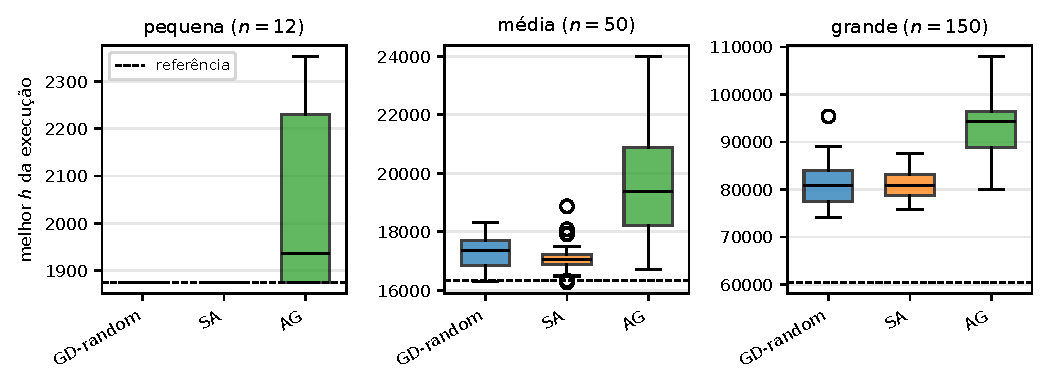
\includegraphics[width=\textwidth]{boxplots}
  \caption{Melhor $h$ por execução. A linha tracejada é o valor de referência da Tabela~\ref{tab:instancias}.}
  \label{fig:boxplots}
\end{figure}

A descida gulosa e o SA não se distinguem estatisticamente em nenhuma instância ($p = 1{,}000$, $0{,}145$ e $0{,}910$).
O SA tem a menor mediana na média e na grande, mas com essa dispersão a diferença não autoriza conclusão.
Os dois vencem o AG nas três instâncias, com $A_{12}$ entre 0,80 e 0,93.
Na grande, onde há só 10 execuções, a vantagem continua significativa ($p$ com Holm de 0,015 e 0,004).
Três execuções na instância média ficaram abaixo da referência publicada: SA com 16\,269, GD-random com 16\,306 e, no experimento extra, o AG memético com 16\,234 (Tabela~\ref{tab:melhores}).
Na grande, a melhor solução que encontramos, 68\,986, ainda está 14\% acima da referência.

\begin{figure}[tbp]
  \centering
  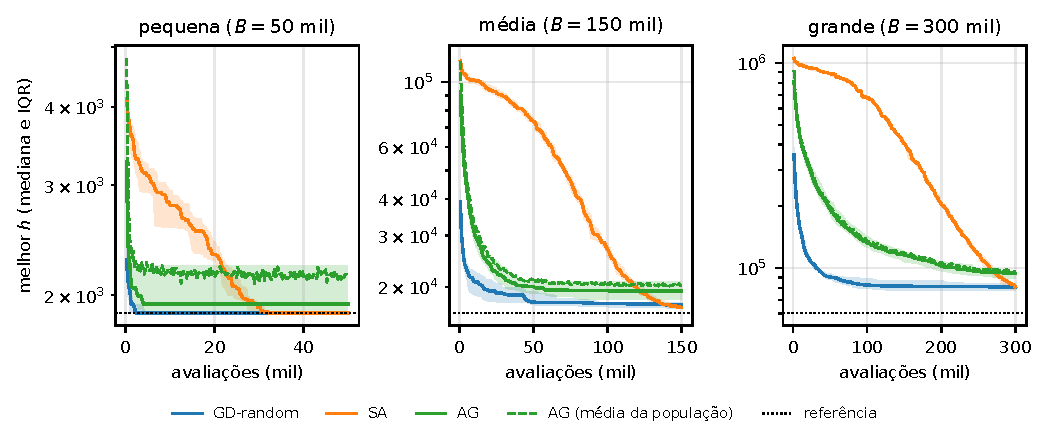
\includegraphics[width=\textwidth]{convergencia}
  \caption{Convergência: mediana (linha) e intervalo interquartil (faixa) do melhor $h$ encontrado até cada avaliação, em escala logarítmica. A linha tracejada verde é a mediana do $h$ médio da população do AG.}
  \label{fig:convergencia}
\end{figure}

As curvas de convergência (Figura~\ref{fig:convergencia}) mostram três dinâmicas diferentes com o mesmo orçamento.
A descida gulosa desce quase toda a distância nas primeiras avaliações e depois avança aos saltos, a cada reinício que encontra um ótimo local melhor.
O SA fica muito acima das outras duas por metade do orçamento, enquanto a temperatura ainda aceita a maior parte das pioras, e só alcança a descida gulosa no fim.
No AG, a curva da média da população passa a acompanhar de perto a do melhor indivíduo depois das primeiras gerações, sinal de que a população ficou homogênea; a distância que sobra, mais visível na pequena, vem dos mutantes criados a cada geração.

\paragraph{Tempo $\times$ avaliações.}
As execuções gastam o mesmo número de avaliações, mas não o mesmo tempo: na grande, 3,8\,s na descida gulosa, 6,0\,s no SA e 8,4\,s no AG, ou cerca de 13, 20 e 28\,µs por avaliação.
O SA também avalia de forma incremental, mas sorteia e calcula uma exponencial a cada passo e reconstrói o prefixo a cada movimento aceito, o que nele acontece com muito mais frequência.
O AG avalia cada filho do zero, porque o filho do OX não compartilha prefixo com uma solução já avaliada, e ainda paga o cruzamento.
Contar avaliações mede o esforço de busca independentemente da implementação e da máquina; com um orçamento de tempo, a vantagem das buscas locais sobre o AG seria ainda maior.

\section{Discussão}
\label{sec:discussao}

\subsection{Ótimos locais e ótimo global}

Na instância pequena, a descida gulosa encontra poucos ótimos locais distintos (Tabela~\ref{tab:otimos}).
Nas 30 execuções, a \textit{best} e a \textit{first improvement} terminaram cerca de 1\,500 e 4\,100 descidas, mas em só 19 permutações diferentes cada uma, e de 11\% a 15,5\% delas terminam no ótimo global.
Com dezenas de reinícios por execução, achar $h^*$ em todas era quase certo.
A paisagem tem poucas bacias, uma delas a do ótimo, o que favorece quem reinicia muitas vezes.
O SA também acha $h^*$ em todas as execuções, por outro caminho: atravessa as barreiras entre bacias aceitando pioras.
O AG acha o ótimo em 12 das 30, porque a população converge antes que algum indivíduo chegue ao fundo da bacia (Seção~\ref{sec:exploracao}).
As 491 paradas distintas da variante \textit{random} não contradizem o quadro: ela para depois de $K$ sorteios sem melhoria, e muitas dessas paradas não são ótimos locais.

\begin{table}[tbp]
  \centering
  \caption{Instância pequena: ótimos locais da descida gulosa (médias por execução, total distinto nas 30 execuções, fração das descidas que terminam em $h^*$) e execuções que atingiram $h^* = 1\,875$.}
  \label{tab:otimos}
  \tabela{otimos_locais}
\end{table}

\subsection{Exploração e intensificação}
\label{sec:exploracao}

Na \textbf{descida gulosa}, o reinício explora e a descida intensifica, e o equilíbrio depende de quantas descidas cabem no orçamento (Tabela~\ref{tab:gd-variantes}).
A \textit{first improvement} completa 10,3 descidas por execução na média e 1,4 na grande.
A \textit{best improvement} paga a vizinhança inteira a cada passo (22\,201 avaliações em $n = 150$) e dá 13 passos de melhoria em 300\,000 avaliações, quando uma permutação aleatória precisa de mais de mil para chegar a um ótimo local.
Na grande, ela termina com mediana de 818\,369,5, pior que o guloso construtivo (398\,095); na média, já perde para as outras variantes ($p = 7{,}0\times10^{-9}$).
A \textit{first} e a \textit{random} dão mais de mil passos por execução e empatam entre si: com orçamento fixo, escolher o melhor sucessor não compensa o preço de examinar todos.

\begin{table}[tbp]
  \centering
  \caption{Variantes da descida gulosa: passos de melhoria, descidas iniciadas e descidas que terminaram em ótimo local (médias por execução), mediana do melhor $h$ e teste contra a variante \textit{random}.}
  \label{tab:gd-variantes}
  \tabela{gd_variantes}
\end{table}

No \textbf{SA}, a temperatura faz a troca.
A aceitação de pioras (Figura~\ref{fig:sa}) começa em 0,87, cai para 0,19 na metade do orçamento e termina entre 0,002 e 0,006, o perfil de passeio aleatório que vira descida que a calibração buscava.
As três curvas praticamente coincidem, embora $T_0$ vá de 5\,481 a 63\,416: calibrar pelo perfil de aceitação neutralizou a diferença de escala de $\Delta$.
O preço está na Figura~\ref{fig:convergencia}: metade do orçamento passa com $h$ muito acima do da descida gulosa, e a última melhoria acontece, na mediana, depois de 98\% do orçamento na média e na grande.
O SA termina ainda melhorando, e com $2B$ foi o que mais ganhou na grande (de 80\,832,5 para 76\,488,5; Tabela~\ref{tab:robustez}).
Na grande, portanto, o equilíbrio pende para a exploração; um $T_0$ menor anteciparia a intensificação, hipótese que não testamos.

\begin{figure}[tbp]
  \centering
  \begin{minipage}[b]{0.335\textwidth}
    \centering
    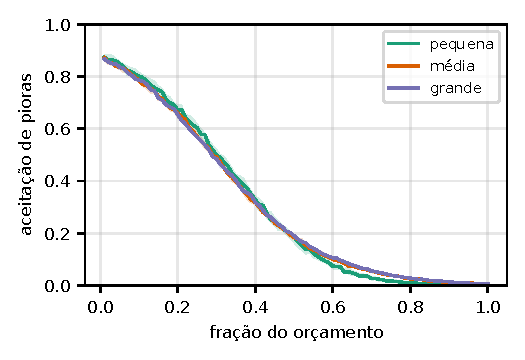
\includegraphics[width=\textwidth]{sa_aceitacao}
  \end{minipage}\hfill
  \begin{minipage}[b]{0.655\textwidth}
    \centering
    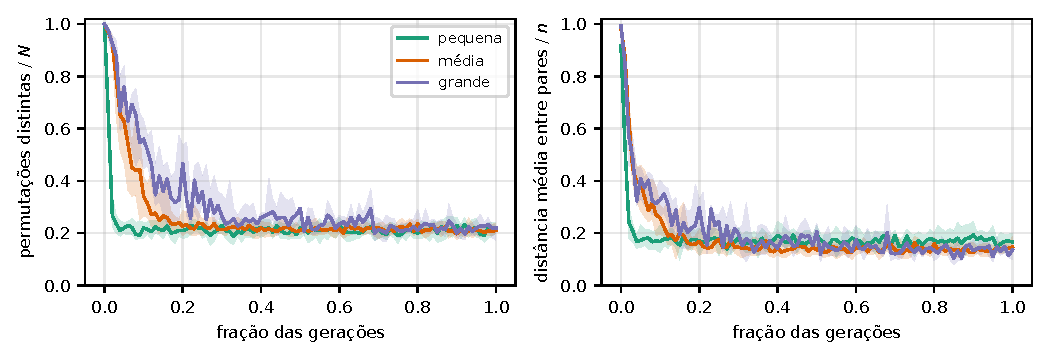
\includegraphics[width=\textwidth]{ag_diversidade}
  \end{minipage}
  \caption{À esquerda, SA: fração das pioras propostas que foram aceitas, por janela de $B/100$ passos. No centro e à direita, AG: permutações distintas como fração de $N$ e distância média entre 50 pares sorteados (posições diferentes) como fração de $n$. Mediana e intervalo interquartil das execuções.}
  \label{fig:sa}
\end{figure}

No \textbf{AG}, a população e o cruzamento exploram, e o torneio com elitismo intensifica.
Aqui o equilíbrio pendeu para a intensificação (Figura~\ref{fig:sa}).
Na pequena, a população de 50 cai para 11 permutações distintas antes de 5\% das gerações, e na média, para um terço em 10\%.
Nas três instâncias a diversidade estaciona perto de 20\%, praticamente os mutantes de cada geração ($P_m = 0{,}2$) em volta de cópias de um indivíduo, e a distância média entre pares cai para cerca de 15\% das posições.
A última melhoria do melhor indivíduo acontece, na mediana, com 3\% do orçamento na pequena e 48\% na média, e na média dar $2B$ ao AG não mudou o resultado de nenhuma das 30 execuções.
Só na grande, onde a população demora mais para convergir, ele ainda melhorava no fim.

\subsection{Efeito de escala}

A ordem não muda com o tamanho: descida gulosa e SA empatados, os dois à frente do AG nas três instâncias.
O que muda é a distância: o gap mediano do AG vai de 3,3\% a 18,7\% e 56\%, e o das buscas locais, de 0 a 4--6\% e 34\%.
Os testes sustentam a ordem só onde há diferença; o empate entre descida gulosa e SA é ausência de evidência de diferença, não evidência de igualdade, e com 10 execuções na grande o teste tem pouco poder.

O custo de examinar a vizinhança explica a maior parte do efeito.
Com $n = 12$, a vizinhança de inserção tem 121 sucessores e uma descida custa algumas centenas de avaliações; com $n = 150$, tem 22\,201 e uma descida custa da ordem de 200\,000.
O orçamento cresce 6 vezes da pequena para a grande, e o espaço de busca, de $10^{8}$ para $10^{262}$ permutações.
A \textit{best improvement}, cujo passo custa $O(n^2)$ avaliações, é a que mais sofre.
O SA não examina vizinhanças e teve a temperatura calibrada por instância, então a escala o atinge menos.
O AG faz poucas gerações para o tamanho do problema e converge longe dos ótimos locais.
Com $2B$ (Tabela~\ref{tab:robustez}) a ordem se manteve: as buscas locais melhoraram, e o AG estacionou na média e continuou atrás na grande.

\subsection{Quando o AG compensa?}

Em nenhuma instância: o AG perde para as duas buscas locais em todas.
O OX aposta que soluções boas compartilham subsequências úteis, como grupos de ativos próximos e com prazos parecidos visitados numa certa ordem, e que cruzar dois pais bons combina blocos bons.
Se a aposta falha, o cruzamento é só uma mutação grande.
Para separar as duas explicações, rodamos o AG em cinco versões, com o mesmo protocolo e as mesmas sementes:
OX (a principal);
PMX~\citep{goldberg1985alleles}, que preserva posições absolutas em vez da ordem relativa;
só mutação ($P_c = 0$);
\textit{headless chicken}~\citep{jones1995crossover}, em que o segundo pai é uma permutação aleatória, o que torna o cruzamento uma macromutação sem informação;
e um AG memético~\citep{moscato1989memetic}, em que cada filho, com probabilidade 0,1 (escolhida num piloto fora do protocolo), desce até um ótimo local por \textit{first improvement}, pagando uma avaliação por sucessor.

\begin{table}[tbp]
  \centering
  \caption{Experimento extra: variantes do AG. Testes de Mann--Whitney contra o AG-OX, com correção de Holm sobre as quatro comparações de cada instância.}
  \label{tab:extra}
  \tabela{extra}
\end{table}

Trocar o OX pelo PMX ou retirar o cruzamento não muda o AG de forma detectável ($p \ge 0{,}275$; Tabela~\ref{tab:extra} e Figura~\ref{fig:extra}, no apêndice), e na grande a versão só com mutação tem até a menor mediana.
O \textit{headless chicken} é muito pior que o OX na média e na grande ($p = 1{,}2\times10^{-10}$ e $7{,}3\times10^{-4}$), pior até que o guloso na grande.
O cruzamento, então, transmite informação do segundo pai, já que trocá-lo por ruído destrói o resultado, mas essa informação não acrescenta nada ao que mutação e seleção fazem sozinhas.
Nossa leitura é que um bloco bom num pai não é bom por si só: seu atraso depende do instante em que a equipe chega a ele, isto é, de tudo o que vem antes na rota.

Só a versão memética melhora o AG, nas três instâncias ($p$ com Holm de $3{,}3\times10^{-6}$, $5{,}6\times10^{-6}$ e $0{,}011$), e ela chega ao nível das buscas locais sem superá-las ($p$ com Holm de 1,000 contra as duas; Tabela~\ref{tab:extra-buscas}).
Com a busca local, o AG vira um gerador de pontos de partida para descidas, e o que ele acrescenta ao reinício aleatório não aparece nos dados.
Neste problema e com este orçamento, o AG não compensa; o que decide é a busca local, venha ela de reinícios, da temperatura ou dos filhos.

\section{Conclusão}
\label{sec:conclusao}

Com orçamento igual e parada exata, a descida gulosa com reinício aleatório e o SA ficaram empatados nas três instâncias, e os dois venceram o AG em todas.
A vizinhança de inserção foi a melhor das três, com o mesmo custo por movimento das outras.
Duas lições do experimento valem além deste problema.
A primeira é que o número de passos de melhoria que cabem no orçamento importa mais que a qualidade de cada passo: a \textit{best improvement} perdeu para variantes que escolhem pior, mas avançam mais.
A segunda é que, neste problema, o cruzamento não combina blocos bons, porque o custo de um bloco depende da posição em que ele cai na rota; o AG só chegou ao nível das buscas locais quando ganhou uma.

Ficam em aberto duas perguntas que os dados sugerem e não testamos.
Uma é se um $T_0$ menor tornaria o SA melhor que a descida gulosa na instância grande, onde ele terminou todas as execuções ainda melhorando.
A outra é se um cruzamento que preserve os instantes de chegada, e não só a ordem, daria ao AG algo que a mutação não dá.


\bibliographystyle{apalike-pt}
\bibliography{referencias}

\appendix
\section{Tabelas e figuras complementares}
\label{ap:tabelas}

\begin{table}[H]
  \centering
  \caption{Calibração do SA por instância. $\Delta^+$ são as pioras observadas entre uma permutação aleatória e um sucessor aleatório.}
  \label{tab:sa-calibracao}
  \tabela{sa_calibracao}
\end{table}

\begin{table}[H]
  \centering
  \caption{T2: testes de Mann--Whitney da inserção contra as outras vizinhanças, com correção de Holm sobre as duas comparações de cada instância.}
  \label{tab:t2-testes}
  \tabela{t2_testes}
\end{table}

\begin{table}[H]
  \centering
  \caption{AG memético contra as duas buscas locais do T3, com correção de Holm sobre as duas comparações de cada instância.}
  \label{tab:extra-buscas}
  \tabela{extra_vs_buscas}
\end{table}

\begin{table}[H]
  \centering
  \caption{Robustez: mediana do melhor $h$ com o orçamento $B$; com $B$ menos as 4\,000 avaliações da calibração (só o SA, com o teste de Mann--Whitney contra o SA com $B$); e com $2B$ na média e na grande, com as mesmas sementes.}
  \label{tab:robustez}
  \tabela{robustez}
\end{table}

Descontar a calibração do orçamento do SA não muda seu resultado de forma detectável ($p = 0{,}515$ na média e $0{,}345$ na grande).
Na grande, porém, a mediana sobe de 80\,832,5 para 82\,246 e passa a ficar acima da descida gulosa (80\,906,5), o que reforça que o SA não é melhor que ela.

\begin{table}[H]
  \centering
  \caption{Parâmetros do AG e mediana de gerações e de permutações distintas na última geração.}
  \label{tab:ag-parametros}
  \tabela{ag_parametros}
\end{table}

\begin{table}[H]
  \centering
  \caption{Melhor solução encontrada por instância em todos os experimentos, reavaliada do zero. As permutações estão em \texttt{relatorio/melhores\_solucoes.txt}.}
  \label{tab:melhores}
  \tabela{melhores}
\end{table}

\begin{figure}[H]
  \centering
  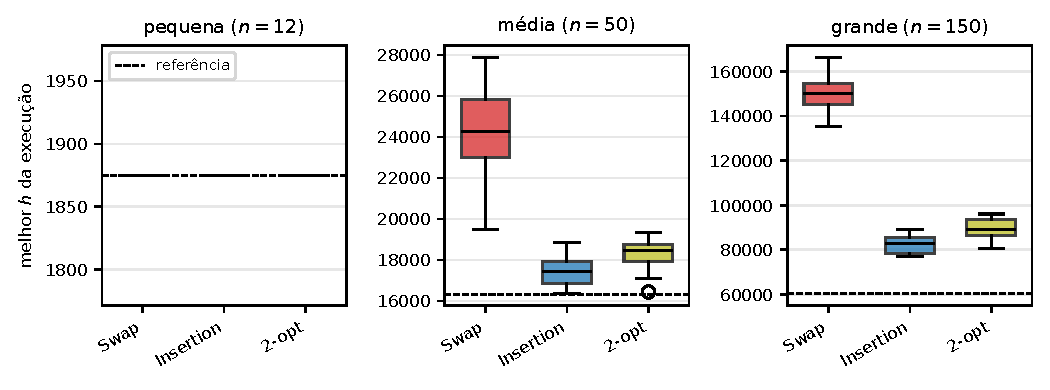
\includegraphics[width=\textwidth]{t2_vizinhancas}
  \caption{T2: melhor $h$ por execução da descida gulosa (\textit{first improvement}) em cada vizinhança.}
  \label{fig:t2}
\end{figure}

\begin{figure}[H]
  \centering
  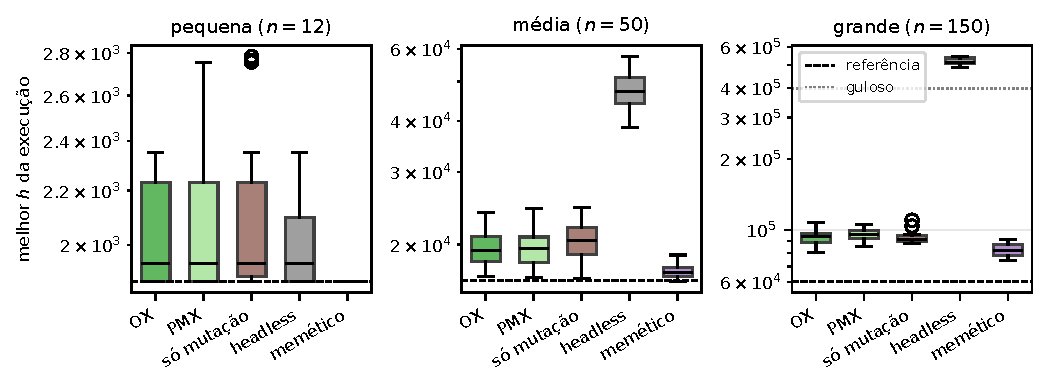
\includegraphics[width=\textwidth]{extra}
  \caption{Experimento extra: melhor $h$ por execução de cada variante do AG (escala logarítmica). A linha pontilhada é o guloso construtivo, desenhada quando cabe na escala.}
  \label{fig:extra}
\end{figure}

\section{Reprodução}
\label{ap:reproducao}

O código acompanha este relatório num arquivo separado, com um README que repete esta tabela.
Pré-requisitos: Python 3.12, \texttt{uv} e \texttt{make}; o primeiro comando é \texttt{make setup}.
Toda execução usa a semente $20\,261\,014 + 1\,000 \cdot i + r$, em que $i$ é o índice da instância e $r$ o da execução, e grava a semente no CSV.

\begin{table}[H]
  \centering\small
  \caption{Comando que gera cada resultado. As pastas de resultados levam a data da execução; as tabelas e figuras usam as pastas indicadas em \texttt{results/LATEST\_*}.}
  \label{tab:reproducao}
  \begin{tabular}{ll}
    \toprule
    Resultado & Comando \\
    \midrule
    Testes automáticos & \texttt{make test} \\
    T1 (saída da Seção~\ref{sec:t1}) & \texttt{make verify} \\
    T2 (execuções e tempo por movimento) & \texttt{make t2} \\
    Calibração do SA (Tabela~\ref{tab:sa-calibracao}) & \texttt{make calibrate} \\
    Exemplo do OX (Tabela~\ref{tab:ox}) & \texttt{make ox-demo} \\
    Pilotos de parâmetros do AG e do AG memético & \texttt{make ag-ajuste memetico-ajuste} \\
    T3 & \texttt{make experiments} \\
    Experimento extra & \texttt{make extra} \\
    Robustez (orçamento sem calibração e $2B$) & \texttt{make robustez} \\
    Tempos sem carga paralela & \texttt{make tempos} \\
    Todas as tabelas e figuras deste relatório & \texttt{make analysis} \\
    Este PDF & \texttt{make report} \\
    \bottomrule
  \end{tabular}
\end{table}


\end{document}
